\documentclass[9pt, aspectratio=169]{beamer}
% \documentclass[10pt]{beamer}
\usepackage[utf8]{inputenc}
\usepackage[T1]{fontenc}
\usepackage[english]{babel}
\usetheme{Frankfurt}

\usepackage[backend=biber, style=authoryear]{biblatex}
\addbibresource{local_references.bib}

%\usepackage{lmodern}
\usepackage{amsfonts,amssymb,amsmath}
\usepackage[english]{babel}
\usetheme{Frankfurt}

\usepackage{csquotes}
\usepackage{setspace}

\usepackage{colortbl}
\usepackage{tabularx}
\renewcommand\tabularxcolumn[1]{m{#1}}

% --- Tickz
\usepackage{physics}
\usepackage{amsmath}
\usepackage{tikz}
\usepackage{mathdots}
\usepackage{yhmath}
\usepackage{cancel}
\usepackage{color}
\usepackage{siunitx}
\usepackage{array}
\usepackage{multirow}
\usepackage{amssymb}
\usepackage{gensymb}
\usepackage{tabularx}
\usepackage{extarrows}
\usepackage{booktabs}
\usetikzlibrary{fadings}
\usetikzlibrary{patterns}
\usetikzlibrary{shadows.blur}
\usetikzlibrary{shapes}

% ---------

\usepackage{booktabs}
\usepackage{setspace}
\usepackage{amssymb}
\usepackage{adjustbox}
\usepackage{pifont}
\usepackage[inkscapeformat=png]{svg}
\usepackage{graphicx}
\usepackage{times}
\setbeamertemplate{caption}[numbered]
% % \setbeamertemplate{bibliography item}{[\theenumiv]}

\setbeamerfont{bibliography item}{size=\tiny}
\setbeamerfont{bibliography entry author}{size=\tiny}
\setbeamerfont{bibliography entry title}{size=\tiny}
\setbeamerfont{bibliography entry location}{size=\tiny}
\setbeamerfont{bibliography entry note}{size=\tiny}

\setbeamerfont{frametitle}{size=\large}

\usepackage{caption}
\usepackage{float}
\usepackage{xcolor}
\usepackage{listings}
\usepackage{animate}

\definecolor{codegreen}{rgb}{0,0.6,0}
\definecolor{codegray}{rgb}{0.5,0.5,0.5}
\definecolor{codepurple}{rgb}{0.58,0,0.82}
\definecolor{backcolour}{rgb}{0.95,0.95,0.92}
 
\lstdefinestyle{mystyle}{
    backgroundcolor=\color{backcolour},   
    commentstyle=\color{codegreen},
    keywordstyle=\color{magenta},
    numberstyle=\tiny\color{codegray},
    stringstyle=\color{codepurple},
    basicstyle=\footnotesize,
    breakatwhitespace=false,         
    breaklines=true,                 
    captionpos=b,                    
    keepspaces=true,                 
    numbers=left,                    
    numbersep=5pt,                  
    showspaces=false,                
    showstringspaces=false,
    showtabs=false,                  
    tabsize=2
}
 
\lstset{style=mystyle}

\usepackage{ragged2e}
\setbeamercolor{section in foot}{fg=white,bg=darkorange}
\setbeamercolor{subsection in foot}{fg=white,bg=darkorange}
\setbeamercolor{frametitle}{fg=white, bg=darkorange}
\setbeamercolor{title}{fg=white, bg=darkorange}
\setbeamercolor{frame}{bg=darkorange}
\setbeamercolor{block title}{bg=darkorange,fg=white}

\setbeamercolor{item}{fg=darkorange}

% \definecolor{darkorange}{rgb}{0.81, 0.52, 0.05}
\definecolor{darkorange}{rgb}{1,0.5,0}
\definecolor{darkorange2}{rgb}{1, 0.64, 0.2}
\definecolor{honeydew}{rgb}{1, 0.85, 0.45}


\newenvironment{variableblock}[3]{%
  \setbeamercolor{block body}{#2}
  \setbeamercolor{block title}{#3}
  \begin{block}{#1}}{\end{block}}

\newenvironment{prosblock}[1]{%
  % \setbeamercolor{block body}{bg=blue,fg=white}
  \setbeamercolor{block title}{bg=blue,fg=white}
  \begin{block}{#1}}{\end{block}}

\newenvironment{consblock}[1]{%
  % \setbeamercolor{block body}{bg=red,fg=white}
  \setbeamercolor{block title}{bg=red,fg=white}
  \begin{block}{#1}}{\end{block}}

\newcommand{\cmark}{\ding{51}}%
\newcommand{\xmark}{\ding{55}}%

\renewcommand{\arraystretch}{1.5}

% Please add the following required packages to your document preamble:
\usepackage{booktabs}
\usepackage{multirow}
\usepackage{colortbl}
% Beamer presentation requires \usepackage{colortbl} instead of \usepackage[table,xcdraw]{xcolor}

\usepackage{tabularray}\UseTblrLibrary{varwidth}
\usepackage{xcolor}
\def\BibTeX{{\rm B\kern-.05em{\sc i\kern-.025em b}\kern-.08em
    T\kern-.1667em\lower.7ex\hbox{E}\kern-.125emX}}
% \usepackage{cite}
\usepackage{amsmath}
\newcommand{\probP}{\text{I\kern-0.15em P}}
\usepackage{etoolbox}
\patchcmd{\thebibliography}{\section*{\refname}}{}{}{}

\setlength\tabcolsep{0.5pt}

\renewcommand{\arraystretch}{0.9}
\setlength{\tabcolsep}{2pt}

\usepackage{pgffor}

\setbeamerfont{bibliography item}{size=\tiny}
\setbeamerfont{bibliography entry author}{size=\tiny}
\setbeamerfont{bibliography entry title}{size=\tiny}
\setbeamerfont{bibliography entry location}{size=\tiny}
\setbeamerfont{bibliography entry note}{size=\tiny}

\setbeamerfont{bibliography entry author}{shape=\upshape,series=\mdseries,size=\footnotesize}
\setbeamerfont{bibliography entry title}{shape=\slshape,series=\mdseries,size=\footnotesize}
\setbeamerfont{bibliography entry journal}{shape=\upshape,series=\mdseries,size=\footnotesize}
\setbeamerfont{bibliography entry note}{shape=\upshape,series=\mdseries,size=\footnotesize}

\renewcommand*{\bibfont}{\scriptsize}

\newenvironment<>{varblock}[2][.9\textwidth]{%
  \setlength{\textwidth}{#1}
  \begin{actionenv}#3%
    \def\insertblocktitle{#2}%
    \par%
    \usebeamertemplate{block begin}}
  {\par%
    \usebeamertemplate{block end}%
  \end{actionenv}}

% \setbeamertemplate{footline}[frame number]

\setbeamertemplate{footline}{
  \leavevmode%
  \hfill
  \usebeamercolor[fg]{page number in head/foot}%
  \scriptsize%
  \ifnum\value{framenumber}>19%
    Appendix \number\numexpr\value{framenumber}-19\relax/32%
  \else%
    \ifnum\value{framenumber}>16%
      %
    \else
      \number\numexpr\value{framenumber}\relax/16%
    \fi

  \fi%
  \hspace{1em}
}


\begin{document}

\author{\textbf{Julien Soulé}, Jean-Paul Jamont, Michel Occello, Paul Théron, Louis-Marie Traonouez}

\title{\textbf{Towards a Multi-Agent Simulation of Cyber-attackers and Cyber-defenders Battles}}

\subtitle{SMC 2023 Presentation}

% \logo{
\includegraphics[scale=0.01]{figures/grenoble-inp_logo.png}}

\institute{\footnotesize \textit{University Grenoble Alpes, Grenoble
INP, LCIS, 26000, Valence, France \\
julien.soule@lcis.grenoble-inp.fr}}

\date{\textit{\footnotesize \today}}

%\subject{}
\setbeamercovered{transparent}
%\setbeamertemplate{navigation symbols}{}
\begin{frame}[plain]
	\maketitle\vspace{-0.8cm}
	\begin{figure}[ht!]
		\centering
            
\includegraphics[height=0.8cm]{figures/la-ruche_logo.png}
            \hspace{0.8cm}
            
\includegraphics[height=0.8cm]{figures/lcis_logo.png}
            \hspace{0.8cm}
		
\includegraphics[height=0.8cm]{figures/grenoble-inp_logo.png}
            \hspace{0.8cm}
            
\includegraphics[height=0.8cm]{figures/uga_logo.jpg}
	\end{figure}
\end{frame}

% \begin{frame}{Content}
%   \tableofcontents
% \end{frame}

\addtocounter{framenumber}{-1}

\section{Introduction}

\begin{frame}{An emergent sense of organization in MARL?}

  \begin{columns}[T]

    \hspace{-0.5cm}
    \begin{column}{0.3\textwidth}

      \vspace{1cm}
      \begin{itemize}
        \item Even without explicit instructions, some distinct behavioral patterns.
        \item In some layouts, these behaviors resemble human-defined \textbf{roles} (and \textbf{goals}).
        \item Yet in others, coordination remains ambiguous.
      \end{itemize}

    \end{column}

    \begin{column}{0.8\textwidth}

      \begin{columns}[T]
        \begin{column}{0.48\textwidth}
          \centering
          \animategraphics[autoplay,loop,width=0.8\linewidth]{8}{figures/overcooked_asymmetric_advantage/frame}{0}{33} \\
          \small{\textbf{Asymmetric Advantage}}\\
          \vspace{0.3em}
          \animategraphics[autoplay,loop,width=0.7\linewidth]{8}{figures/overcooked_coordination_ring/frame}{0}{33} \\
          \small{\textbf{Coordination Ring}}
        \end{column}
        \begin{column}{0.48\textwidth}
          \centering
          \animategraphics[autoplay,loop,width=0.75\linewidth]{8}{figures/overcooked_counter_circuit/frame}{0}{33} \\
          \small{\textbf{Counter Circuit}}\\
          \vspace{0.3em}
          \animategraphics[autoplay,loop,width=0.7\linewidth]{8}{figures/overcooked_forced_coordination/frame}{0}{33} \\
          \small{\textbf{Forced Coordination}}
        \end{column}
      \end{columns}

    \end{column}

  \end{columns}

  \hspace{-1cm}
  \vspace{-0.5cm}
  {\tiny \textit{Overcooked-AI~\autocite{overcookedai}}}

\end{frame}


\appendix
%\setbeamertemplate{headline}{}
\setbeamertemplate{mini frames}{}

% \AtBeginSection[]{
% 	\begin{frame}
% 		\frametitle{}
% 		\tableofcontents[currentsection]
% 	\end{frame}
% }

% %%%%%%%%%%%%%%%%%%%%%%%%%%%%%%%%%%%%

\section*{\phantom{Thanks}}

\begin{frame}{}

  \vspace{6ex}

  \centering
  {
    \Huge
    \emph{Thank You}
  }

  \vspace{6ex}

  \begin{columns}

    \hspace{-27ex}

    \begin{column}{0.5\textwidth}
      \raggedleft
      {\Large Demo video $\Longrightarrow$}
    \end{column}

    \hspace{-12ex}

    \begin{column}{0.5\textwidth}
      
\includegraphics[width=0.5\linewidth]{figures/demo_qr_code.png}
    \end{column}

  \end{columns}

  \vspace{3ex}

  \centering
  {\Large
    \url{https://t.ly/4JBxr}
  }

\end{frame}

% \AtBeginSection[]{
% 	\begin{frame}
% 		\frametitle{}
% 		\tableofcontents[currentsection]
% 	\end{frame}
% }

% %%%%%%%%%%%%%%%%%%%%%%%%%%%%%%%%%%%%

\section*{\phantom{References}}

\begin{frame}[allowframebreaks]{References}{}
    
    % \bibliographystyle{plain}
    % \bibliography{local_references}
        
    \printbibliography

\end{frame}

\newcounter{mainframenumber}
\setcounter{mainframenumber}{\value{framenumber}}

% \begin{frame}[allowframebreaks]{Annexes} {Contexte}

    \begin{block}{Paradigme des Systèmes Multi-Agents (SMA) pour des problèmes complexes et distribués}
        \begin{itemize}
            \item \textbf{décomposition des tâches} : missions déléguées aux agents réalisées par coopération~\parencite{Raileanu2023} ;
            \item \textbf{avantages} : gérer des objectifs contradictoires, calcul parallèle, robustesse du système, évolutivité\dots
        \end{itemize}
    \end{block}
    
    \begin{block}{\textbf{Organisation} : clé pour la conception des SMA}
        \begin{itemize}
            \item \textbf{coordination} : comment atteindre un objectif commun de manière collaborative~\parencite{Hubner2007} ;
            \item \textbf{environnements dynamiques et incertains} : comportement flexible à l'exécution pour s'adapter~\parencite{Kathleen2020} ;
        \end{itemize}
    \end{block}
    
    \begin{block}{Méthodes et pratiques pour la conception des SMA}
        \begin{itemize}
            \item \textbf{approche + modèle organisationnel} : les méthodes s'appuient sur l'expérience des concepteurs pour concevoir manuellement les \textbf{politiques} des agents afin que le SMA atteigne ses objectifs ;
                  %   \begin{itemize}
                  %       \item Exemples : \emph{GAIA}~\parencite{Wooldridge2000,Cernuzzi2014}, \emph{ADELFE}~\parencite{Mefteh2015}, ou \emph{DIAMOND}~\parencite{Jamont2015}, \emph{KB-ORG}~\parencite{Sims2008}
                  %   \end{itemize}
            \item \textbf{simulation vers la réalité} : 1) conception sûre et efficace des SMA dans un environnement simulé à haute fidélité ; \quad 2) transfert à un environnement réel pour des performances adéquates~\parencite{Schon2021}.
        \end{itemize}
        \quad $\Longrightarrow$ \textbf{Processus itératif par essais et erreurs}
    \end{block}

\end{frame}

\begin{frame}[allowframebreaks]{Annexes} {Fondamentaux des SMA}

    \begin{block}{Mots-clés}
        \begin{itemize}
            \item \textbf{Agent} : entité immergée dans un environnement, percevant des observations et prenant des décisions de manière autonome pour atteindre des objectifs ;
            \item \textbf{SMA} : ensemble d'agents collaborant avec des mécanismes d'auto/réorganisation pour atteindre leurs objectifs ;
            \item \textbf{Organisation} : interactions des agents même si elles peuvent être implicites ;
            \item \textbf{Modèle organisationnel (OM)} : moyen de décrire formellement une organisation explicite/implicite ;
            \item \textbf{Spécifications organisationnelles (OS)} : composants d'un OM pour caractériser une organisation.
        \end{itemize}
    \end{block}
    
    \begin{block}{Modèle organisationnel : $\mathcal{M}OISE^+$}
        \begin{itemize}
            \item plus complexe que \emph{Agent Group Roles} (intégration des normes) ;
            \item prend explicitement en compte les aspects sociaux entre les agents ;
            \item permet de lier les politiques des agents aux spécifications organisationnelles.
        \end{itemize}
    \end{block}

\end{frame}

\begin{frame}[allowframebreaks]{Annexes} {Fondamentaux du MARL}

    \begin{block}{Mots-clés}
        \begin{itemize}
            \item \textbf{Politique} : la \textquote{logique} pour choisir la prochaine action en fonction de l'observation pour un agent ;
            \item \textbf{Historique/trajectoire} : le couple (observation, action) sur un épisode ;
            \item \textbf{Politique/historique conjoints} : l'ensemble des politiques/historiques de tous les agents sous forme de tuples ;
            \item \textbf{Apprentissage par renforcement} : un agent met à jour sa politique pour maximiser une récompense cumulative ;
            \item \textbf{Apprentissage par renforcement multi-agent (MARL)} : extension à plusieurs agents qui apprennent en prenant en compte les actions des autres agents ;
        \end{itemize}
    \end{block}
    
\end{frame}

\begin{frame}[allowframebreaks]{Annexes}{Approche AOMEA : Fondement théorique}
    \begin{block}{MARL orienté organisation (OMARL)}
        Un processus de MARL augmenté avec un OM pour :
        \begin{itemize}
            \item \textbf{Contraindre l'espace des politiques} : obtenir les politiques conjointes satisfaisant les spécifications de conception données ;
            \item \textbf{Inférer des spécifications organisationnelles} : obtenir des spécifications à partir des politiques des agents.
        \end{itemize}
    \end{block}
    
    \begin{block}{Algorithme \emph{Partial Relations with Agent History and Organization Model} (PRAHOM)}
        Implémentation d'un processus OMARL\dots
        \begin{enumerate}
            \item \textbf{Contraindre l'espace des politiques}
                  \begin{itemize}
                      \item Impossible d'utiliser directement les politiques $\rightarrow$ \textbf{historiques} caractérisant les \textbf{politiques} ;
                      \item Relations entre \textbf{OS} et historiques attendus ;
                      \item Les agents contraints aux OS $\rightarrow$ à chaque étape : actions disponibles mises à jour en fonction des historiques \textbf{OS}.
                  \end{itemize}
    
            \item \textbf{Inférer des spécifications organisationnelles}
                  \begin{itemize}
                      \item Analyser les historiques $\rightarrow$ caractériser les comportements collectifs comme OS ;
                      \item Utilisation des relations connues entre OS et historiques ;
                      \item Utilisation de la définition générale des OS par rapport aux historiques.
                  \end{itemize}
        \end{enumerate}
    \end{block}
    
\end{frame}

\begin{frame}{Annexes}{Aperçu de \textit{PRAHOM}}
    \begin{figure}
        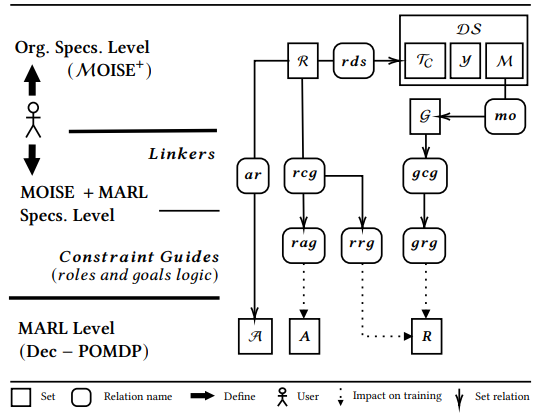
\includegraphics[width=0.6\linewidth]{figures/mm_simple_representation.png}
    \end{figure}
\end{frame}
    
\begin{frame}{Annexes}{Aperçu de PRAHOM}
    \begin{figure}
        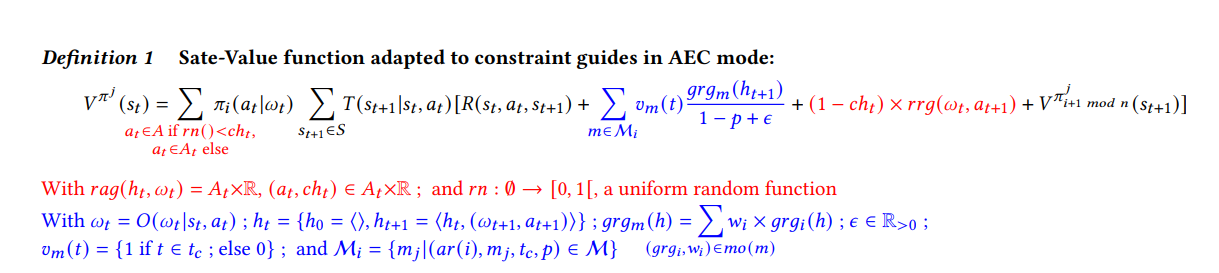
\includegraphics[width=\linewidth]{figures/modified_state_value_function.png}
    \end{figure}
\end{frame}
    
\begin{frame}[allowframebreaks]{Annexes}{Approche AOMEA : Fondement théorique}
    \textbf{Contraindre l'espace des politiques} pendant l'entraînement

    \begin{columns}
    
        \begin{column}{0.3\textwidth}
    
            \begin{itemize}
                \item À chaque étape, l'ensemble des actions disponibles est modifié pour correspondre aux contraintes de politiques définies par les utilisateurs ;
                \item Contraintes intégrées via : correction externe, apprentissage, modification interne des politiques.
            \end{itemize}
    
        \end{column}
    
        \begin{column}{0.8\textwidth}
            \begin{figure}
                \centering
                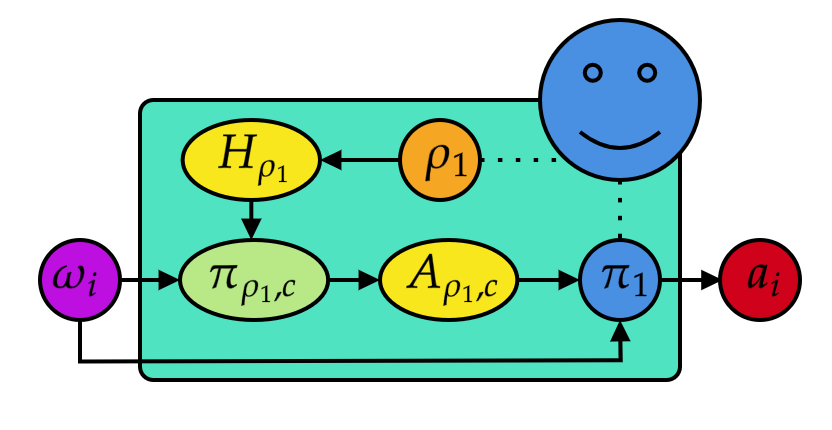
\includegraphics[width=0.7\linewidth]{figures/prahom_training_constrain.png}
                \caption*{Vue résumée de la contrainte PRAHOM}
                \label{fig:prahom_process}
            \end{figure}
        \end{column}
    
    \end{columns}
\end{frame}

\begin{frame}{Annexes}{Constrained Reinforcement Learning (Constrained-RL)}
    
    \begin{itemize}
        \item Apprendre une politique optimisant la récompense tout en respectant des \textbf{contraintes de sécurité} ou de \textbf{performance}.
        
        \item \textbf{Contraintes dures} : doivent toujours être respectées (Shielding).
        \item \textbf{Contraintes douces} : respectées en moyenne ou sous forme de pénalités.
        
        \item \textbf{Méthodes :}
            \begin{itemize}
                \item \textbf{Reward Shaping} : ajout de pénalités pour violation de contraintes.
                \item \textbf{Policy Projection} : ajustement des actions pour rester dans les limites.
                \item \textbf{Dual Variables} : intégration de multiplicateurs de Lagrange pour gérer les contraintes.
            \end{itemize}
            
    \end{itemize}    
\end{frame}

\begin{frame}{Annexes}{Safe Exploration et Shielding en Reinforcement Learning}
    
    \begin{itemize}
        \item \textbf{Safe Exploration} $\rightarrow$ garantir la sécurité lors de la phase d'exploration en limitant les risques de comportements dangereux.
        \item Principalement modifier la fonction de récompense (Langragien) pour integrer contraintes mais aussi\dots
        \item \textbf{Shielding} intervenir en temps réel pour bloquer les actions susceptibles de violer ces contraintes, permettant une exploration sécurisée.
    \end{itemize}
    
    \textbf{Référence :} \\
    \textit{Akifumi Wachi, Wataru Hashimoto, Xun Shen, \& Kazumune Hashimoto (2023). Safe Exploration in Reinforcement Learning: A Generalized Formulation and Algorithms. In Thirty-seventh Conference on Neural Information Processing Systems.}

\end{frame}

\begin{frame}[allowframebreaks]{Annexes}{Approche AOMEA: Fondement théorique}

    \textbf{Inferrer des Spécifications Organisationnelles}

    \begin{columns}

        \begin{column}{0.3\textwidth}

            \begin{itemize}
                \item \textbf{Knowledge-based Organizational Specifications Identification (KOSIA)}
                \item \textbf{General Organizational Specifications Infererence (GOSIA)}
            \end{itemize}

        \end{column}

        \begin{column}{0.8\textwidth}
            \begin{figure}
                \centering
                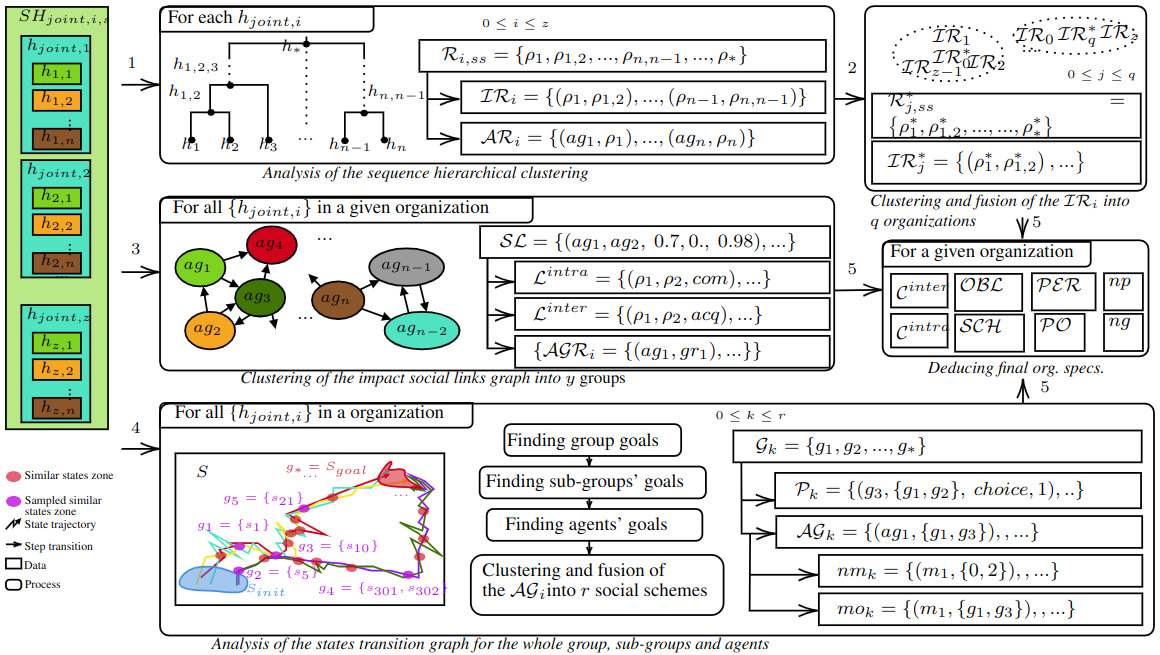
\includegraphics[width=0.95\linewidth]{figures/GOSIA_view.png}
                \caption*{A summary view of the GOSIA process}
                \label{fig:gosia_process}
            \end{figure}
        \end{column}

    \end{columns}

\end{frame}


%%%%%%%%%%%%%%%%

% Slide 2: Exemple d'utilisation
\begin{frame}[fragile]{Annexes}{Exemple d'utilisation d'Optuna}
    \begin{itemize}
        \item \textbf{Optuna} est une bibliothèque open-source pour l'optimisation des hyperparamètres (HPO), utile en apprentissage automatique.
        \item Exemples d'hyper-paramètre : taux d'apprentissage, fonction activation, nb couche, taille couches, seuil de ressemblance pour Hierarchical Clustering\dots
        \item \textbf{Étapes pour utiliser Optuna :}
        \begin{itemize}
            \item \texttt{1.} Définir une fonction d'objectif.
            \item \texttt{2.} Lancer une étude avec Optuna.
            \item \texttt{3.} Utiliser le meilleur résultat pour entraîner le modèle.
        \end{itemize}
    \end{itemize}

    \begin{lstlisting}[language=Python, basicstyle=\small\ttfamily, frame=single, caption=Exemple d'Optuna en Python]
import optuna

def objective(trial):
    x = trial.suggest_float("x", -10, 10)
    return (x - 2) ** 2 # Mock : fonction "etat-valeur"

study = optuna.create_study(direction="minimize")
study.optimize(objective, n_trials=100)

print(study.best_params)  # Affiche les meilleurs parametres
    \end{lstlisting}
\end{frame}


\begin{frame}{Annexes}{Aperçu PettingZoo}
    \begin{itemize}
        \item Bibliothèque Python pour environnements multi-agents.
        \item Simplifier l'entraînement et l'évaluation des agents dans divers environnements.
        \item \textbf{Caractéristiques principales} :
        \begin{itemize}
            \item Supporte plusieurs types d'environnements multi-agents (tour par tour, simultané, etc.).
            \item Intégration facile avec des frameworks de reinforcement learning comme RLlib.
            \item Compatible avec les API de Gym, permettant une utilisation intuitive.
        \end{itemize}
        \item \textbf{Exemples d'environnements inclus} :
        \begin{itemize}
            \item Jeux : \textit{TicTacToe}, \textit{ConnectFour}.
            \item Scénarios de collaboration et de compétition : \textit{Pistonball}, \textit{Prisoner's Dilemma}.
            \item Intégration avec la suite d'environnements Atari pour le multi-agent.
        \end{itemize}
    \end{itemize}
\end{frame}

\begin{frame}[fragile]{Annexes}{Exemple utilisation de PettingZoo}
    \begin{itemize}
        \item Exemple : Création et interaction avec un environnement.
        \item Chargement de l'environnement, réinitialisation et étapes d'interaction pour un agent.
    \end{itemize}
    \vspace{0.3cm}
    \begin{lstlisting}[language=Python, basicstyle=\ttfamily\small]
from pettingzoo.butterfly import pistonball_v6

# Creer et reinitialiser l'environnement
env = pistonball_v6.env()
env.reset()

# Boucle principale d'interaction
for agent in env.agent_iter():
    obs, reward, done, info = env.last()
    action = env.action_space(agent).sample()  # Action aleatoire
    env.step(action)
    if done:
        env.reset()  # Reinitialiser si l'episode est termine
\end{lstlisting}
\end{frame}


\begin{frame}{Annexes}{KB-Org}
    \frametitle{Organization-based multi-agent systems: From modeling to implementation}
    
    \begin{itemize}
        \item Modélisation et mise en œuvre des SMA basés sur organisation ;
        \item Intègre les concepts d'organisation pour structurer les interactions et le comportement des agents ;
        \item Banque d'organisations disponibles prêtes à être utilisé ;
        \item Explicabilité et à la coordination.
    \end{itemize}
    
    \

    Sims, V. (2008). Automated organization design for multi-agent systems. Autonomous Agents and Multi-Agent Systems, 16(2), 151-185.

\end{frame}

\begin{frame}{Annexes}{Présentation de la bibliothèque MARLlib}

    \begin{itemize}
        \item Bibliothèque Python pour MARL
        \item Supporte plusieurs environnements MARL comme PettingZoo, StarCraft II, MPE (Multi-Agent Particle Environment), etc.
        \item Implémente divers algorithmes MARL, incluant MADDPG, MAPPO, etc.
        \item Fournit une interface pour comparaison d’algorithmes, l’entraînement et l’évaluation.
        \item Offre des configurations \textit{fine-tunés} pour de nombreux environnements
    \end{itemize}

\end{frame}

\begin{frame}[allowframebreaks]{Annexes}{Présentation de la bibliothèque MARLlib}

    \begin{itemize}
        \item \textbf{Algorithmes Basés sur les Valeurs}  
        \begin{itemize}
            \item \textbf{Multi-Agent Q-Learning} : Une extension multi-agent fondamentale de Q-learning.  
            \textit{Description} : Simple à implémenter, mais avec des difficultés de scalabilité et de non-stationnarité.
            \item \textbf{MADDPG} : Une adaptation de DDPG pour les environnements multi-agents.  
            \textit{Description} : Gère bien les espaces d'actions continues, mais requiert beaucoup de données et est complexe.
        \end{itemize}
    
        \

        \item \textbf{Algorithmes Basés sur les Politiques}  
        \begin{itemize}
            \item \textbf{REINFORCE} : Une méthode de gradient de politique basique pour l'apprentissage direct de la politique.  
            \textit{Description} : Adaptable aux environnements stochastiques mais souffre de variances élevées des gradients.
            \item \textbf{Multi-Agent PPO (MAPPO)} : Une extension de PPO conçue pour les configurations multi-agents.  
            \textit{Description} : Stabilise les mises à jour, mais nécessite un ajustement minutieux et un coût de calcul élevé.
        \end{itemize}
    
        \item \textbf{Algorithmes Hybrides}  
        \begin{itemize}
            \item \textbf{A3C (Asynchronous Advantage Actor-Critic)} : Combine l'apprentissage des politiques et des valeurs pour un équilibre exploration/exploitation.  
            \textit{Description} : Accélère l'entraînement mais nécessite une synchronisation complexe.
            \item \textbf{MAPPO} : Un hybride intégrant PPO avec un entraînement centralisé.  
            \textit{Description} : Efficace pour les tâches coopératives, mais difficile dans les environnements compétitifs et exigeant en ressources.
        \end{itemize}
    
        \item \textbf{Algorithmes Théoriques et Coopératifs Basés sur le Jeu}  
        \begin{itemize}
            \item \textbf{Independent Q-Learning (IQL)} : Une version indépendante de Q-learning pour chaque agent.  
            \textit{Description} : Simple à implémenter mais avec de sérieux problèmes de non-stationnarité en multi-agent.
            \item \textbf{COMA (Counterfactual Multi-Agent Policy Gradients)} : Utilise des baselines contrefactuelles pour évaluer les contributions des agents.  
            \textit{Description} : Réduit la variance et améliore la coopération, mais demande des calculs lourds.
        \end{itemize}
    
        \item \textbf{Entraînement Centralisé avec Exécution Décentralisée}  
        \begin{itemize}
            \item \textbf{QMIX} : Décompose les valeurs Q pour améliorer la coordination multi-agent.  
            \textit{Description} : Équilibre l'entraînement centralisé et l'action décentralisée, mais moins efficace en environnements très compétitifs.
            \item \textbf{VDN (Value Decomposition Networks)} : Simplifie la coordination multi-agent avec la décomposition des valeurs.  
            \textit{Description} : Efficace mais limité dans la gestion d'interactions complexes.
        \end{itemize}
    \end{itemize}
    

\end{frame}


\end{document}
